	\documentclass[12pt]{book}
\usepackage[a4paper, total={6in, 8in}]{geometry}
\usepackage{amssymb}
\usepackage{listings}
\usepackage{color}
\usepackage{graphicx}
\usepackage{subfig}
\usepackage{float}
\definecolor{mygrey}{gray}{.96} % Light Grey
\definecolor{BrickRed}{RGB}{120,0,0}


\def\xbf{\mathbf{x}}
\def\zbf{\mathbf{z}}
\def\xibf{\mathbf{\xi}}
\lstset{
	language=R,              % choose the language of the code ("language=Verilog" is popular as well)
   tabsize=3,							  % sets the size of the tabs in spaces (1 Tab is replaced with 3 spaces)
	basicstyle=\footnotesize,               % the size of the fonts that are used for the code
	numbers=left,                   % where to put the line-numbers
	numberstyle=\footnotesize,              % the size of the fonts that are used for the line-numbers
	stepnumber=1,                   % the step between two line-numbers. If it's 1 each line will be numbered
	numbersep=5pt,                  % how far the line-numbers are from the code
	backgroundcolor=\color{mygrey}, % choose the background color. You must add \usepackage{color}
	showspaces=false,              % show spaces adding particular underscores
	showstringspaces=false,        % underline spaces within strings
	showtabs=false,                % show tabs within strings adding particular underscores
	frame=single,	                 % adds a frame around the code
	tabsize=3,	                    % sets default tabsize to 2 spaces
	captionpos=b,                   % sets the caption-position to bottom
	breaklines=true,                % sets automatic line breaking
	breakatwhitespace=false,        % sets if automatic breaks should only happen at whitespace
	%escapeinside={\%*}{*)},        % if you want to add a comment within your code
	commentstyle=\color{BrickRed}   % sets the comment style
}

\begin{document}
\title{\textbf{Monte Carlo Simulation Lab Assignment-10}}	
\author{Yash Vanjani\\140123046\\Mathematics and Computing\\IIT Guwahati}
\date{April 18 , 2016}

\maketitle

\newpage


\newpage
\begin{enumerate}
\item[Q 1]  a financial asset. The process ${S(t)}$ is a $GBM$ with drift parameter $\mu$, volatility parameter $\sigma$, and initial value $S(0)$ if \newline
$S(t) = S(0)exp([\mu-\frac{\sigma^2}{2}]t + \sigma W(t)).$ \newline
where ${W(t)}$ is a standard BM. As with the case of a BM, we have a simple
recursive procedure to simulate a GBM at $0=t_0 < t_1 < ... t_n$ as \newline
$S(t_{i+1} = S(t_i) exp([\mu - \frac {\sigma^2}{2}] (t_{i+1}-t_i) + \sigma
\sqrt{t_{i+1}-t_i}Z_{i+1})$ \newline
where $Z_1 , Z_2 ,..., Z_n$ are independent $N (0, 1)$ variates. In the
interval $[0, 5],$ taking both positive and negative values for $\mu$ and for at
least two different values of $\sigma^2$ , simulate and plot at least $10$ sample
paths of the GBM (taking sufficiently large number of sample points for each path).
Also, by generating a large number of sample paths, compare the actual and simulated
distributions of $S(5)$. Calculate expectation and variance of $S(5)$ and match it
with the theoretical values.\\
\end{enumerate}

\textbf{Solution} 


\noindent{Code for R}

\begin{lstlisting}
library(stats)
S<-vector("numeric")
t<-vector("numeric")
pal<- palette()
t[1]=0
sec5<-vector("numeric") #for storing BM values at 5th sec
mu<-(1.2)#mu=mean
sigma<-0.6 #sigma=standard deviation

for(i in 1:4999)
{
	t[i+1]=t[i]+0.001
}
for(i in 1:10)
{
	z<-rnorm(5000, mean=0, sd=1)
	S[1]=1
	for (j in 1:4999)
	{
		S[j+1]=S[j]*exp(((mu-(sigma*sigma/2))*(0.001))+(sigma*z[j+1]*sqrt(0.001)))
		if(j==4999)
		{
			sec5[i]=S[5000]
		}

	}
	if(i==1)
	{
		plot(t,S,type="l", col=pal[i %% 8 +1],ylim=c(0,600))
	}
	else
	{
		lines(t,S, col=pal[i %% 8 +1],ylim=c(0,600))
	}
}
cat("\nFor S(t=0) = ",S[1],", mu = ",mu,", var = ",(sigma*sigma),"\n")
cat("experemntal E[S(5)] = ",mean(sec5),"\n")
cat("experemntal Var[S(5)] = ",var(sec5),"\n")
mu_theoritical<-S[1]*exp(mu*5)
var_theoritical<-S[1]*S[1]*exp(2*mu*5)*(exp(sigma*sigma*5)-1)
cat("theoritical E[S(5)] = ",mu_theoritical,"\n")
cat("theoritical Var[S(5)] = ",var_theoritical,"\n\n")
\end{lstlisting}
\newpage

The above code is run for both positive and negative values of $\mu$ and three different values of $\sigma ^2$.


\textbf{1) $\mu=-1$ and $\sigma ^2=0.0009$}\\\\
\begin{lstlisting}
	experemntal E[S(5)] =  0.006568828 
	experemntal Var[S(5)] =  1.110003e-07 
	theoritical E[S(5)] =  0.006737947 
	theoritical Var[S(5)] =  2.0476e-07 
\end{lstlisting}
The corresponding plot obtained is shown below:
\begin{figure}[H]
	\centering
	\subfloat[For $\mu=-1 ,\sigma ^2=0.0009$]{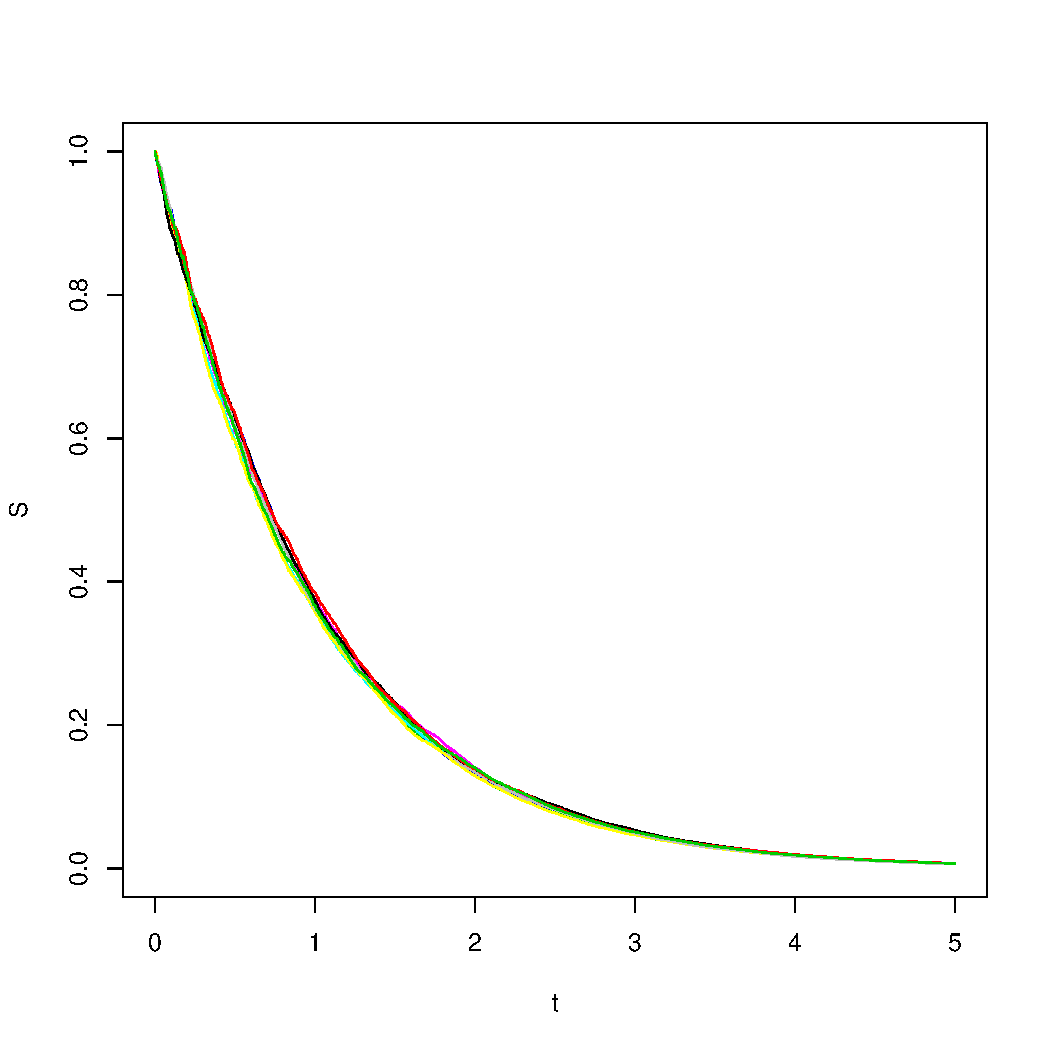
\includegraphics[width=0.8\textwidth]{1.pdf}}	
\end{figure}
\newpage
\textbf{2) $\mu=-1$ and $\sigma ^2=0.16$}\\\\
\begin{lstlisting}
	experemntal E[S(5)] =  0.007180603 
	experemntal Var[S(5)] =  3.251476e-05 
	theoritical E[S(5)] =  0.006737947 
	theoritical Var[S(5)] =  5.563947e-05 
\end{lstlisting}
The corresponding plot obtained is shown below:
\begin{figure}[H]
	\centering
	\subfloat[For $\mu=-1 ,\sigma ^2=0.16$]{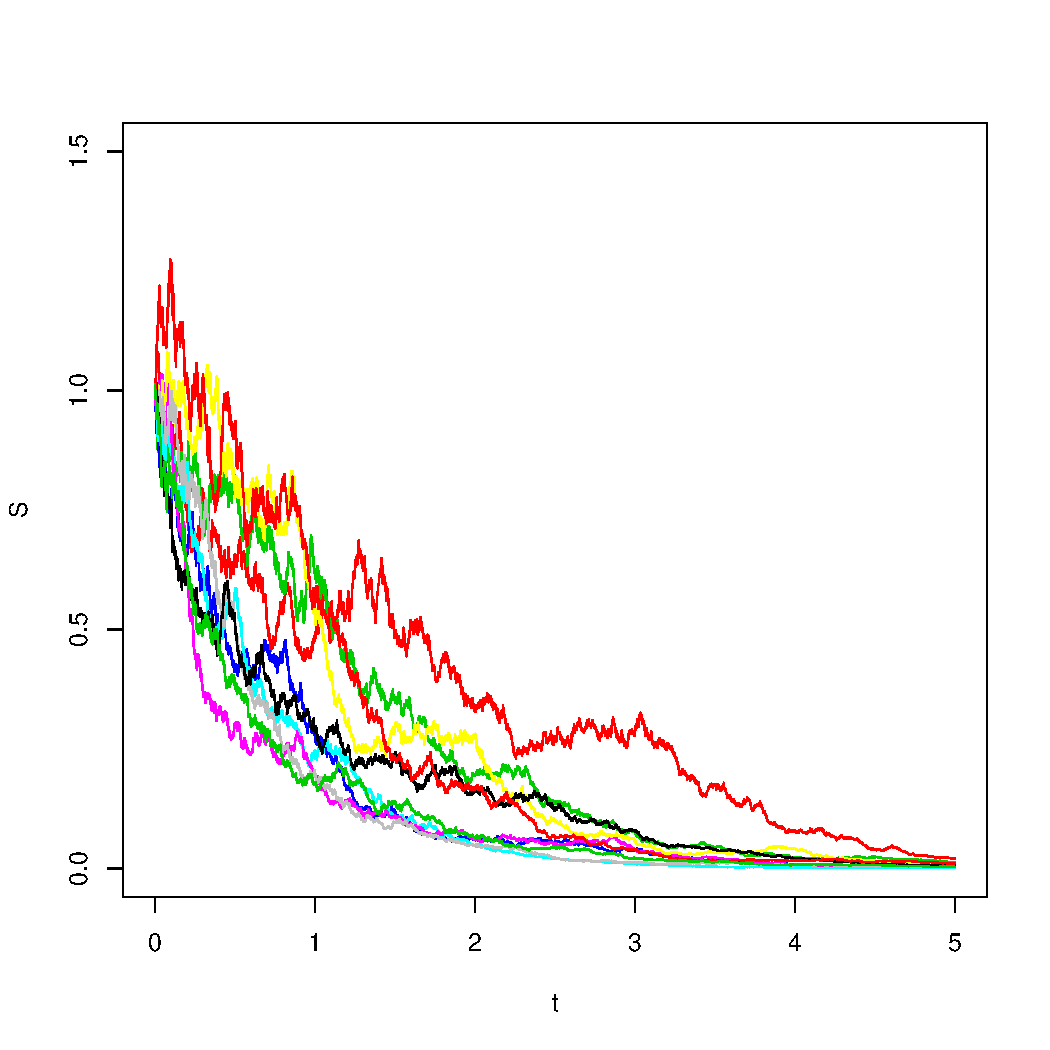
\includegraphics[width=0.8\textwidth]{2.pdf}}	
\end{figure}
\newpage
\textbf{3) $\mu=-1$ and $\sigma ^2=0.64$}\\\\
\begin{lstlisting}
	experemntal E[S(5)] =  0.001537008 
	experemntal Var[S(5)] =  3.101096e-06 
	theoritical E[S(5)] =  0.006737947 
	theoritical Var[S(5)] =  0.001068375 
\end{lstlisting}
The corresponding plot obtained is shown below:
\begin{figure}[H]
	\centering
	\subfloat[For $\mu=-1 ,\sigma ^2=0.64$]{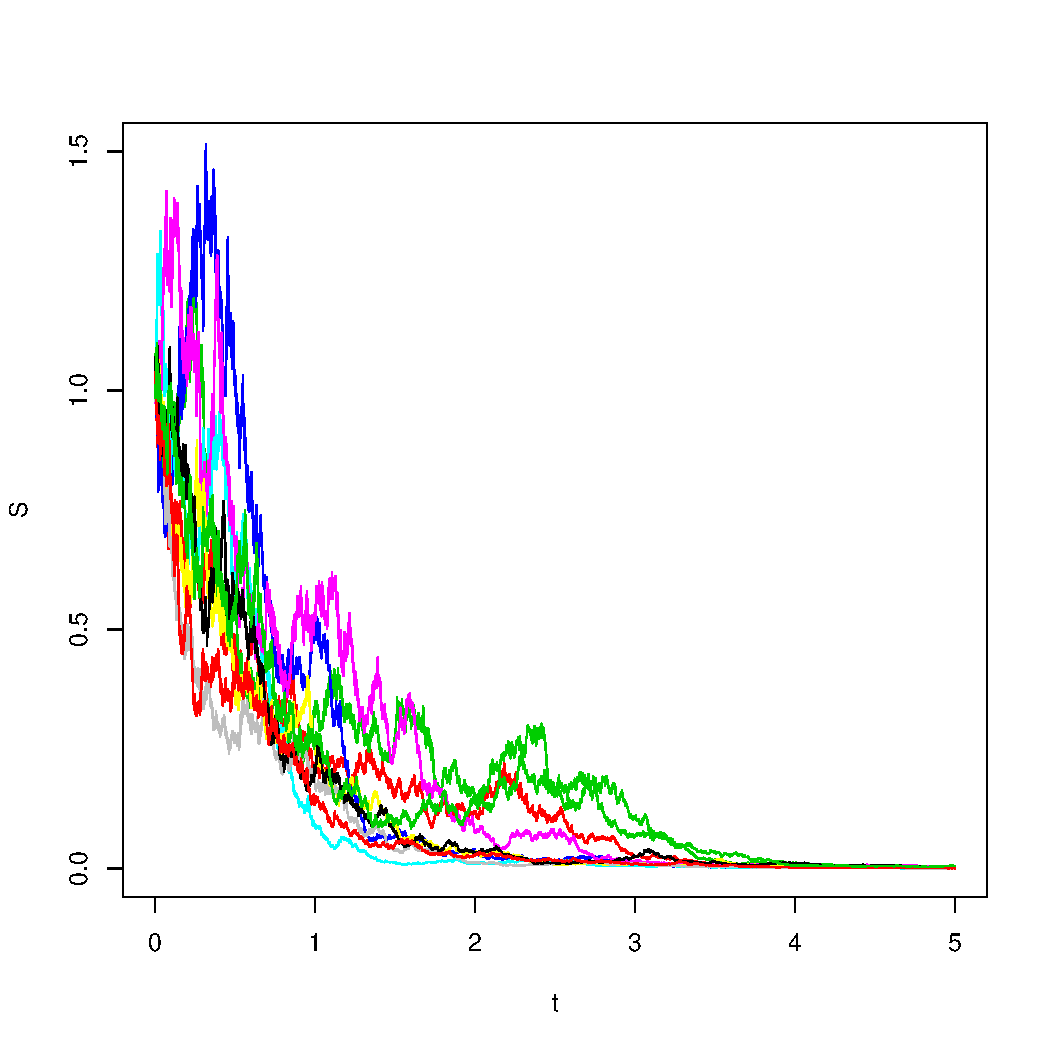
\includegraphics[width=0.8\textwidth]{3.pdf}}	
\end{figure}
\newpage
\textbf{4) $\mu=0.1$ and $\sigma ^2=0.0009$}\\\\
\begin{lstlisting}
	experemntal E[S(5)] =  1.640698 
	experemntal Var[S(5)] =  0.01144312 
	theoritical E[S(5)] =  1.648721 
	theoritical Var[S(5)] =  0.01225983
\end{lstlisting}
The corresponding plot obtained is shown below:
\begin{figure}[H]
	\centering
	\subfloat[For $\mu=0.1 ,\sigma ^2=0.0009$]{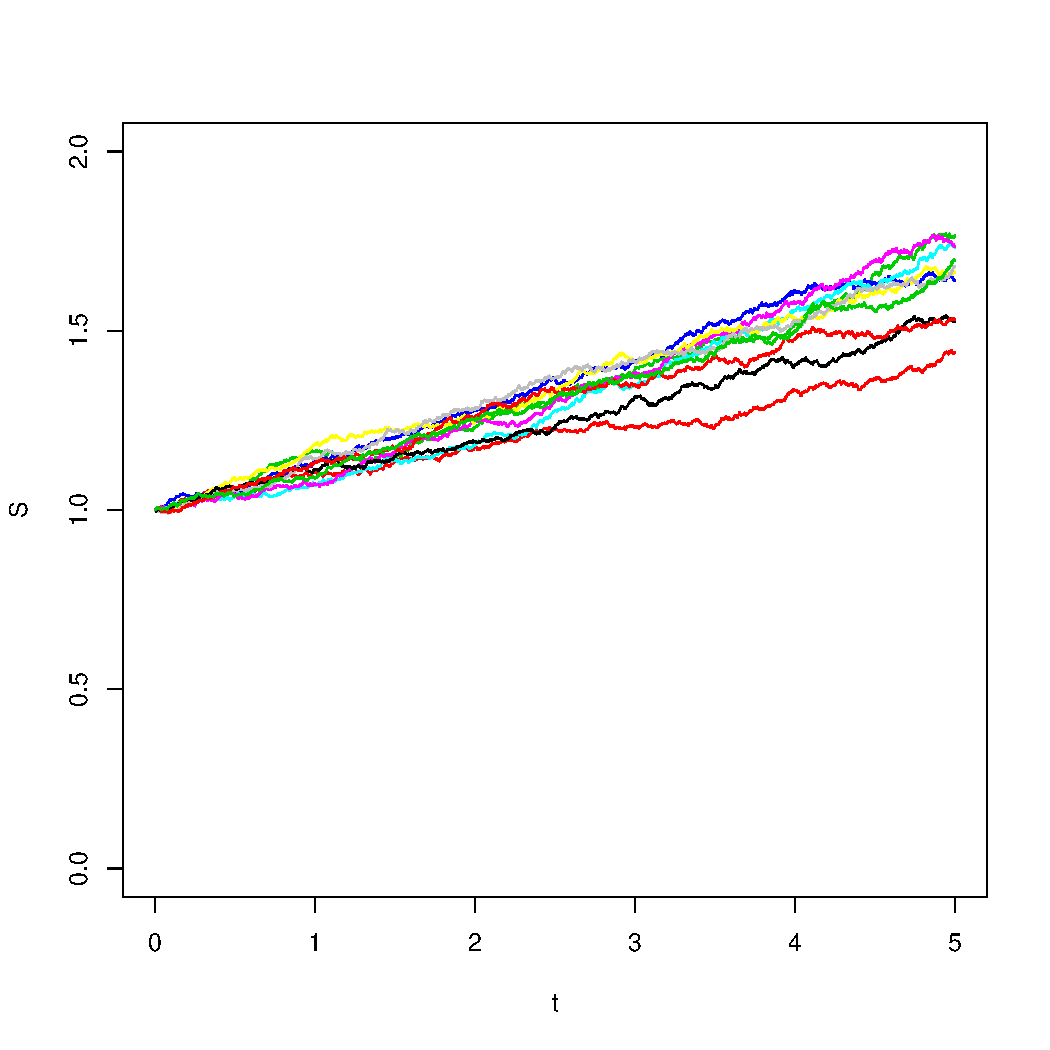
\includegraphics[width=0.8\textwidth]{4.pdf}}	
\end{figure}
\newpage
\textbf{5) $\mu=0.1$ and $\sigma ^2=0.16$}\\\\
\begin{lstlisting}
	experemntal E[S(5)] =  1.965153 
	experemntal Var[S(5)] =  3.815481 
	theoritical E[S(5)] =  1.648721 
	theoritical Var[S(5)] =  3.331366 
\end{lstlisting}
The corresponding plot obtained is shown below:
\begin{figure}[H]
	\centering
	\subfloat[For $\mu=0.1 ,\sigma ^2=0.16$]{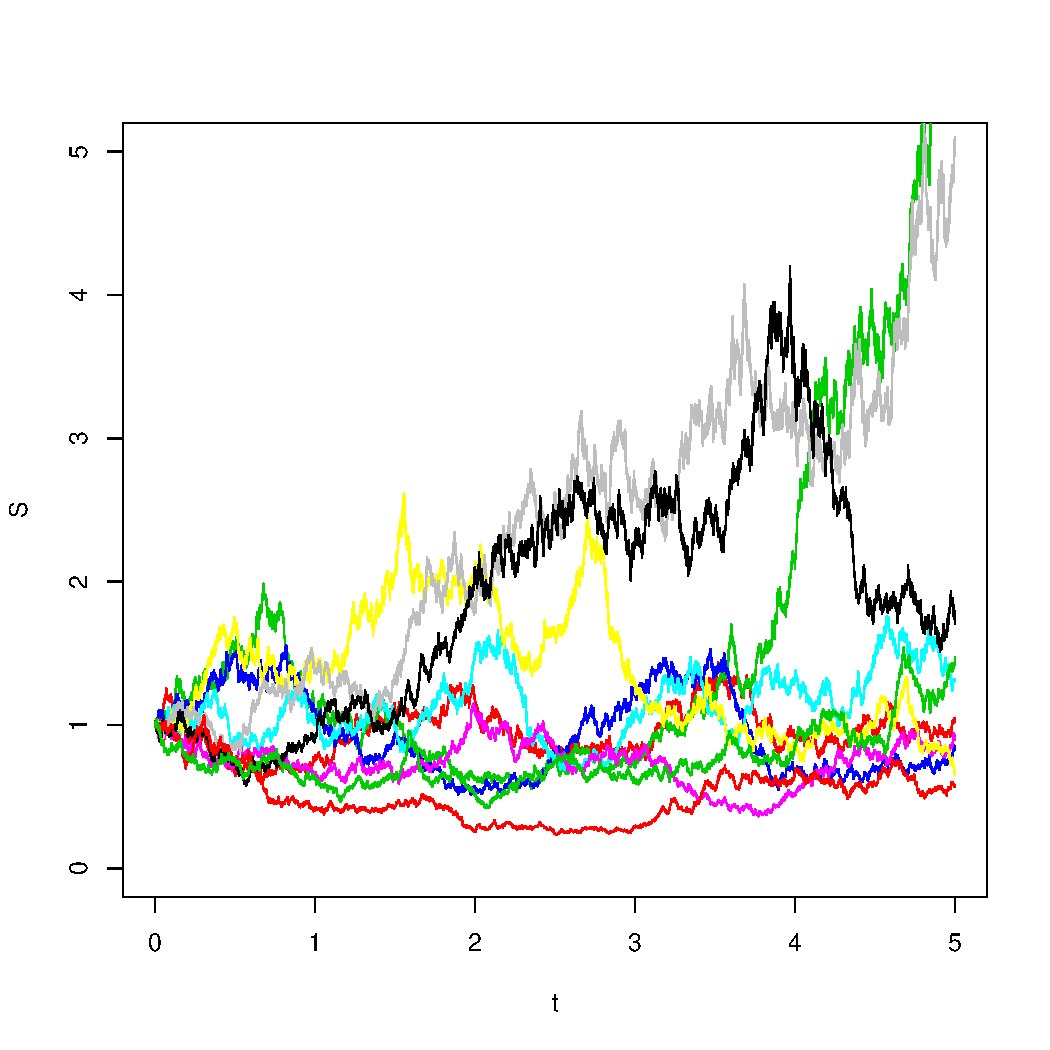
\includegraphics[width=0.8\textwidth]{5.pdf}}	
\end{figure}
\newpage
\textbf{6) $\mu=0.1$ and $\sigma ^2=0.36$}\\\\
\begin{lstlisting}
	experemntal E[S(5)] =  2.060723 
	experemntal Var[S(5)] =  13.35654 
	theoritical E[S(5)] =  1.648721 
	theoritical Var[S(5)] =  13.72636 
\end{lstlisting}
The corresponding plot obtained is shown below:
\begin{figure}[H]
	\centering
	\subfloat[For $\mu=0.1 ,\sigma ^2=0.36$]{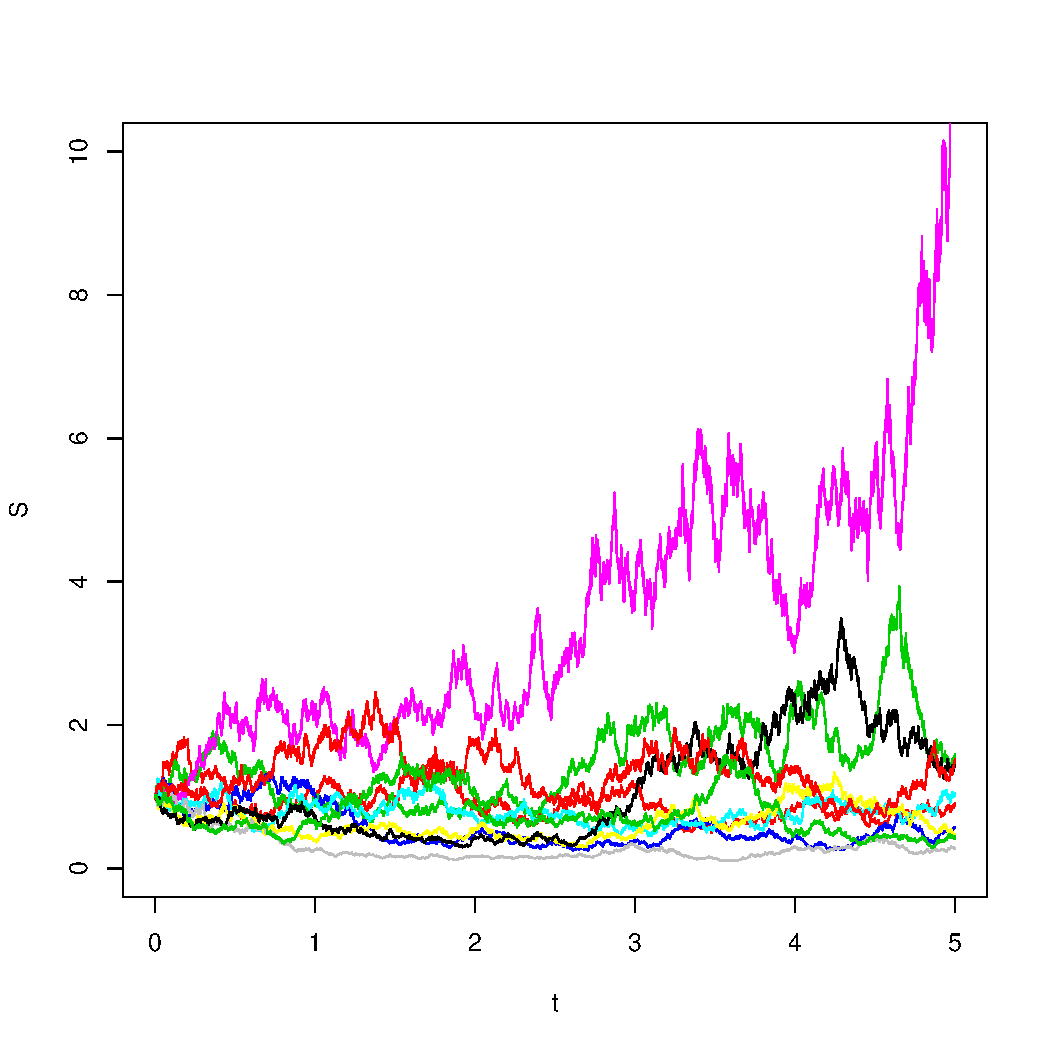
\includegraphics[width=0.8\textwidth]{6.pdf}}	
\end{figure}
\newpage
\textbf{7) $\mu=1.2$ and $\sigma ^2=0.0009$}\\\\
\begin{lstlisting}
	experemntal E[S(5)] =  389.121 
	experemntal Var[S(5)] =  759.7764 
	theoritical E[S(5)] =  403.4288 
	theoritical Var[S(5)] =  734.0469 
\end{lstlisting}
The corresponding plot obtained is shown below:
\begin{figure}[H]
	\centering
	\subfloat[For $\mu=1.2 ,\sigma ^2=0.0009$]{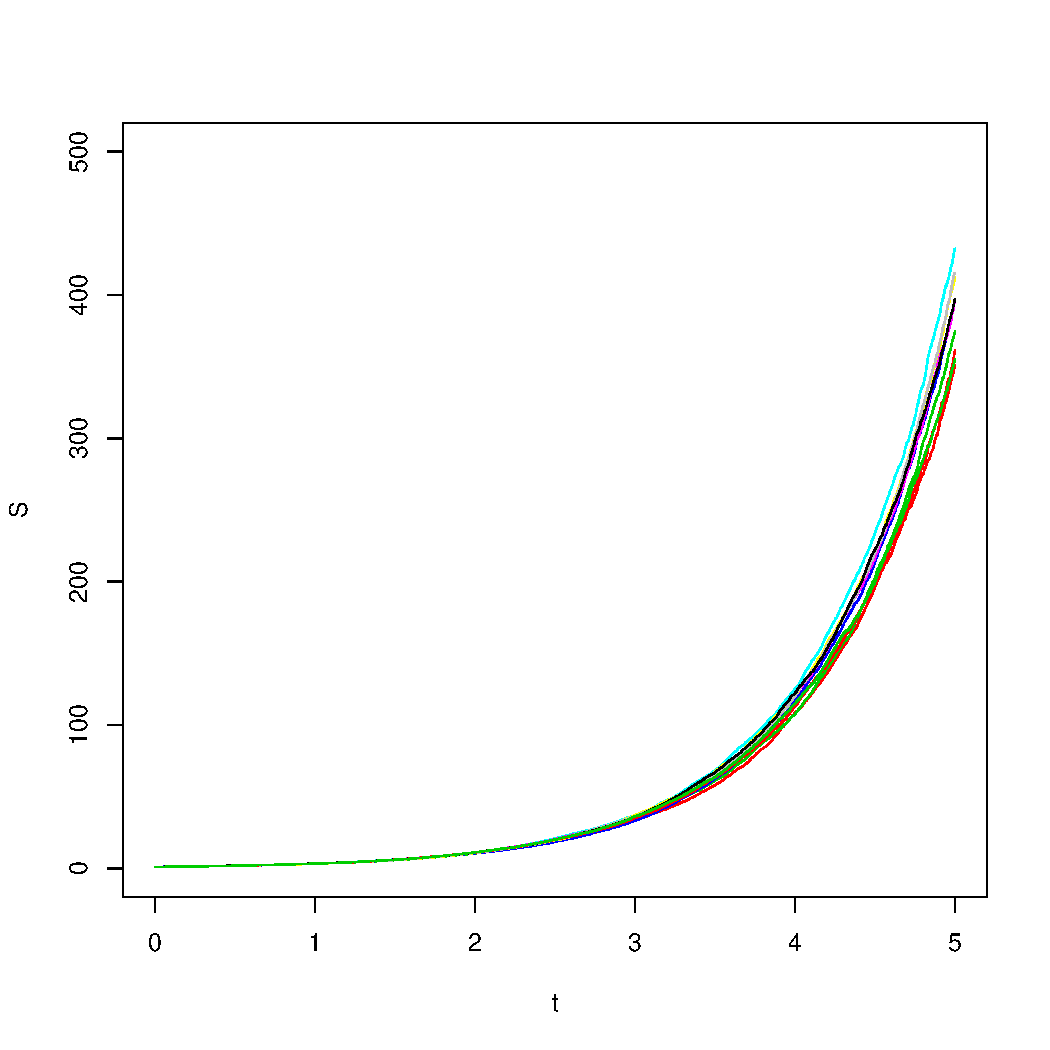
\includegraphics[width=0.8\textwidth]{7.pdf}}	
\end{figure}
\newpage
\textbf{8) $\mu=1.2$ and $\sigma ^2=0.16$}\\\\
\begin{lstlisting}
	experemntal E[S(5)] =  481.3793 
	experemntal Var[S(5)] =  143927.7 
	theoritical E[S(5)] =  403.4288 
	theoritical Var[S(5)] =  199462.7 
\end{lstlisting}
The corresponding plot obtained is shown below:
\begin{figure}[H]
	\centering
	\subfloat[For $\mu=1.2 ,\sigma ^2=0.16$]{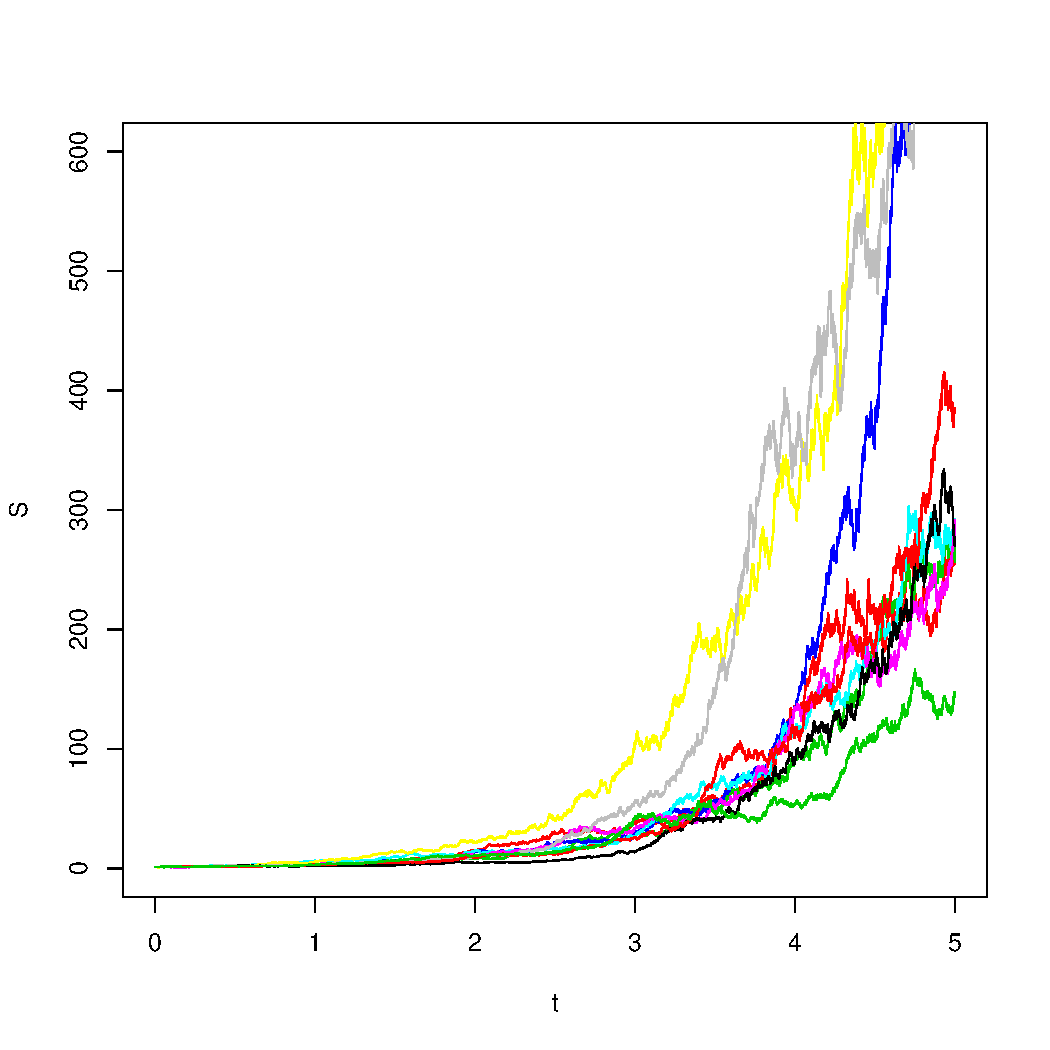
\includegraphics[width=0.8\textwidth]{8.pdf}}	
\end{figure}
\newpage
\textbf{9) $\mu=1.2$ and $\sigma ^2=0.36$}\\\\
\begin{lstlisting}
	experemntal E[S(5)] =  343.1025 
	experemntal Var[S(5)] =  77828.83 
	theoritical E[S(5)] =  403.4288 
	theoritical Var[S(5)] =  821854.3 
\end{lstlisting}
The corresponding plot obtained is shown below:
\begin{figure}[H]
	\centering
	\subfloat[For $\mu=1.2 ,\sigma ^2=0.36$]{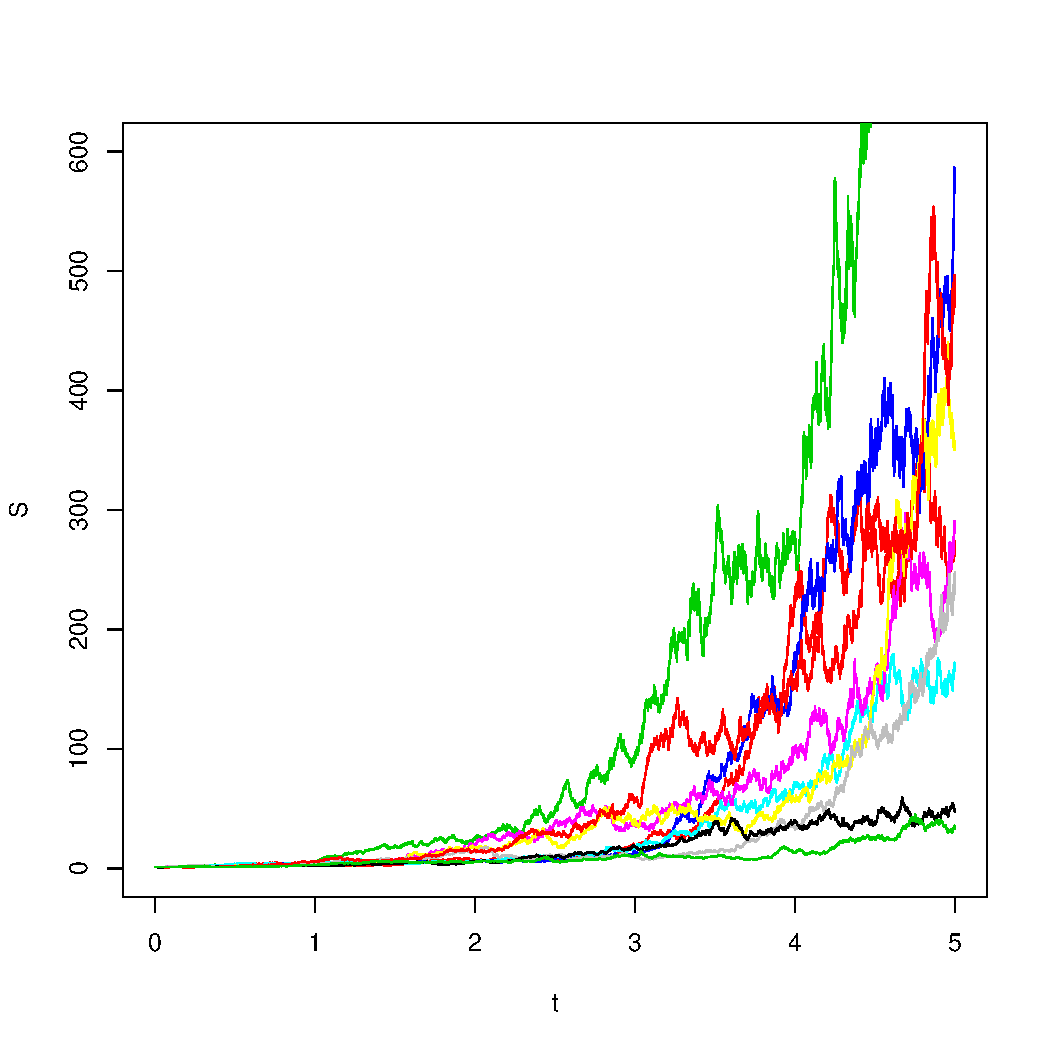
\includegraphics[width=0.8\textwidth]{9.pdf}}	
\end{figure}

\end{document}
